The mean free path of tritium electrons in water is only around $5~\mu\meter$, so most electrons emitted in tritiated water do not reach the scintillating fibres. These electrons do not provide useful information and only consume computing resources. To optimize the simulation, the dimensions of the simulated tritium source were set to maximize the number of tritium events reaching the scintillating fibres. The distribution of the initial energy of tritium electrons capable of penetrating a fibre and depositing energy, shown in Figure \ref{subfig:EnergySpectrumEventsDetectedandNonDetected}, is shifted to high energies and has a peak centred at $10~\keV$. 

\begin{figure}
\centering
    \begin{subfigure}[b]{0.6\textwidth}
    \centering
    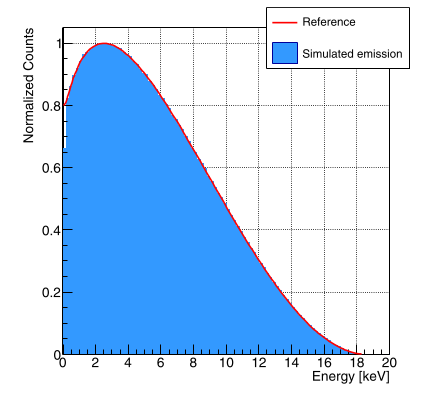
\includegraphics[width=\textwidth]{6Simulations/61TRITIUMDesign/611TritiumSourceOptimization/TritiumSourceEnergyDistribution.png}  
    \caption{\label{subfig:EnergyDistributionTritiumSource}}
    \end{subfigure}
    \hfill
    \begin{subfigure}[b]{0.6\textwidth}
    \centering
    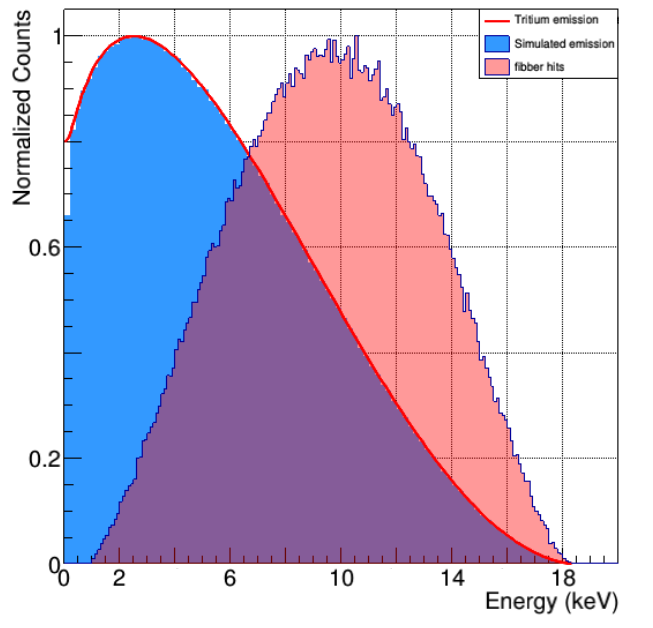
\includegraphics[width=\textwidth]{6Simulations/61TRITIUMDesign/611TritiumSourceOptimization/Source_Spectrum_yes_and_non_detected_events.png}  
    \caption{\label{subfig:EnergySpectrumEventsDetectedandNonDetected}}
    \end{subfigure}
 \caption{Energy distribution of a) simulated tritium decays b) Initial energy of tritium decays that reach the scintillating fibres (red histogram) compared to all simulated tritium events (blue histogram) \cite{SimulationPaperCarlos}.
 \label{fig:TritiumSourceOptimization}}
\end{figure}

A $20~\cm$ long and $2~\mm$ diameter scintillating fibre surrounded by a tritiated water source of the same length and $0.5~\mm$ thickness ($100$ times greater that the mean free path of tritium electrons) were simulated. Only the energy deposition of tritium electrons in the fibre was registered, excluding optical processes. The goal of these simulations was to find the radial thickness of the simulated tritium source beyond which no significant amount of tritium decay electrons are detected. In Figure \ref{subfig:TransversalCutTritiumSource}, a transversal cut of the $2~\mm$ scintillating fibre, the $0.5~\mm$ thick tritium source surrounding the fibre and the positions where happen the tritium decays that deposit energy in the scintillating fibre are shown. Furthermore, the distribution of the radial distance between the position where tritium decays take place and the surface of the scintillating fibre is shown in figure \ref{subfig:DistanceDistributionTritiumSourceFiber}. The thickness of the simulated tritium source was $5~\mu\meter$ since $99.4\%$ of the events that deposit energy in the fibres are produced at a shorter distance. These results are independent of the fibre diameter.

\begin{figure}
\centering
    \begin{subfigure}[b]{0.5\textwidth}
    \centering
    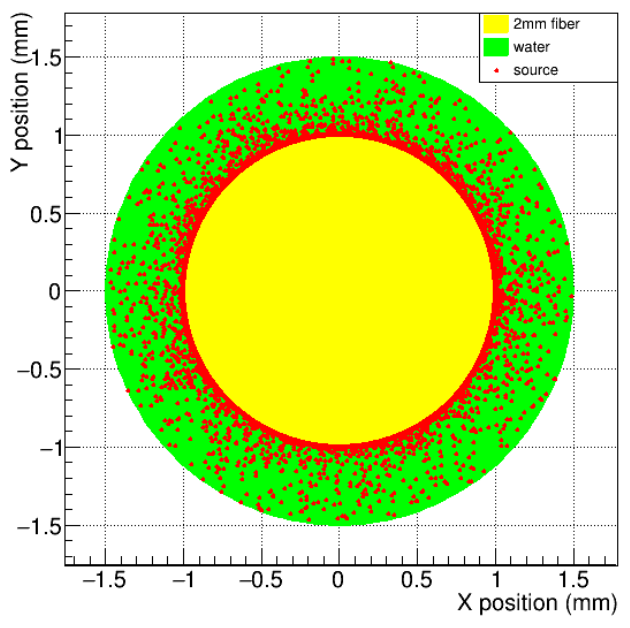
\includegraphics[width=\textwidth]{6Simulations/61TRITIUMDesign/611TritiumSourceOptimization/Source_Ring.png}  
    \caption{\label{subfig:TransversalCutTritiumSource}}
    \end{subfigure}
    \hfill
    \begin{subfigure}[b]{0.5\textwidth}
    \centering
    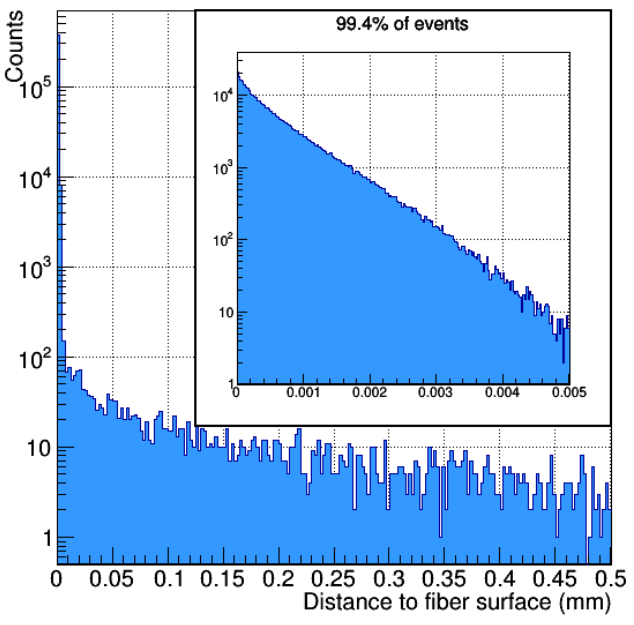
\includegraphics[width=\textwidth]{6Simulations/61TRITIUMDesign/611TritiumSourceOptimization/SourceDistance.png}  
    \caption{\label{subfig:DistanceDistributionTritiumSourceFiber}}
    \end{subfigure}
 \caption{a) Cross seccion of a simulated scintillating fibre (yellow) and the tritium source (green) with various tritium decays (red dots) b) Distribution of the radial distance between the position where the tritium decays take place and the surface of the scintillating fibre \cite{SimulationPaperCarlos}. A zoom of low energy events is shown in the inset.}
 \label{fig:TritiumSourceSimulated}
\end{figure}	

